\documentclass{article}
\usepackage{blindtext}
\usepackage[margin=0.75in]{geometry}
\usepackage[utf8]{inputenc}
\usepackage{amsmath}
\usepackage{stackengine}
\usepackage[pdftex]{graphicx}
\usepackage{float}
\usepackage{newlfont}
\usepackage{amssymb}
\usepackage{verbatim} 
\usepackage[final]{pdfpages}
\usepackage{setspace}
\setlength{\parindent}{0pt}

\title{Multi-Armed Bandit Problem}
\author{Sunith Suresh, Lin Xiao, Ilan Man and Sanjay Hariharlaan}
\date{\today} 
\begin{document}
\maketitle

\section{Introduction}

This paper explores the multi-armed bandit problem (MAB). A multi-armed bandit is a sequential experiment with the goal of achieving the largest possible reward from a payoff distribution with unknown parameters. The term multi-armed bandit comes from slot machines where each machine is known as a one-armed bandit. In this set up, at each iteration the player must decide which arm of the experiment to observe next.\\

The task is complicated by the stochastic nature of the bandits in the following two ways:

\begin{enumerate}
\item A suboptimal bandit can return many winnings, purely by chance, which would make us believe that it is a very profitable bandit. Similarly, the best bandit might not yield a reward if only played a few times.
\item If we have a found a bandit that returns pretty good results, do we keep drawing from it to maintain our pretty good score, or do we try other bandits in hopes of finding an even-better bandit? How do we know when to switch and when to stick to the current bandit? This is the \textit{exploration vs. exploitation} dilemma.
\end{enumerate}

This algorithm is popular in machine learning literature as an example of reinforcement learning, as well as game theory as an example of optimal decision making in the face of multiple choices.\\

This paper reviews several strategies for selecting machines, including a novel (to our knowledge) approach using dynamic programming, and compares each approach against each other. Note that there are variations on the stochastic MAB, including contextual bandit and adverserial bandit, which we will not discuss here.

\section{Multi-armed bandit review}

In Machine Learning literature, the stochastic multi-armed bandit problem is formulated as:

\begin{quote}
Given $K$ machines, each with an unknown probability of yielding a reward, which come from a fixed but unknown distribution parameterized by $\theta_i$, for $i \in (1, ..., K)$, and $N$ total plays, decide which machines to play in order to maximize the total reward.
\end{quote}

It is common in the literature to express the maximum reward as minimzing \textit{regret} compared to the best arm in hindsight. That is, define regret at each step as $r_{t} = R^* - R_{i}$, where $R^*$ is the reward yielded by selecting the best machine and $R_{i}$ is the reward yielded by selecting machine $i$. The goal is then to devise a strategy to minimize $\sum_{t=1}^N r_{t}$. Note that since this is a stochastic problem, we aim to minimize regret in expectation or with high probability.\\

The common theme between the algorithms outlined in this paper are that our objective is to select the optimal machine to play at each time step, given that we want to minimize cumulative regret. The approach to selecting which machine to play is known as the \textit{policy} or acquisition function, denoted as $U(\alpha_i, \beta_i)$. This function balances the trade off between selecting the best machine based on previous plays and the possibility of a better machine that hasn't been selected yet.

\section{Dynamic Programming}


We begin our analysis by constructing a simple approach to maximizing Future Expected Rewards. Consider the Bernoulli Bandit case.

We designate the following:

$$R_1 = \text{Reward from Machine 1} \sim \text{Bernoulli}(\theta_1)$$
$$R_2 = \text{Reward from Machine 2} \sim \text{Bernoulli}(\theta_2)$$

$$\theta_1 \sim \text{Beta}(\alpha_1, \beta_1)$$
$$\theta_2 \sim \text{Beta}(\alpha_2, \beta_2)$$

In the beginning, we have no prior knowledge about either Machine, or more specifically, about the latent parameter governing each Machine. Therefore, we initially set $\alpha_1, \alpha_2, \beta_1, \beta_2 = 1$. 

Given our goals above, the main question becomes: **How do we choose which Machine to play in each Iteration?** We will refer to this question as our utility or acquisition function $U(\theta | X) = U(\alpha_1, \beta_1, \alpha_2, \beta_2 | X)$.

As we begin playing and gathering information, we continuously update our parameters of interest based on the outcome. Specifically:

1. $U(\alpha_1, \beta_1, \alpha_2, \beta_2) = j$ 
    * ( We choose Machine j )
2. $R_j = i$  
    * ( We play Machine j, and get Reward i )
3. If $R_j = 1$:
    $\alpha_j = \alpha_j + 1$  
4. If $R_j = 0$:
    $\beta_j = \beta_j + 1$  

The idea is to update our prior belief on the success of the individual Machines based on our empirical rewards. $\alpha$ represents success, while $\beta$ represents failure

Before we discuss how to construct our Acquisition Function $U(\theta|X)$ which will help us decide which Machine to play at each iteration, we see two interesting points:

At time T = 1, we have no prior belief concerning any Machine. Thus, it will not matter which Machine we pick the first time around, though it will influence all subsequent choices.

At time T = N, we are at our final trial, and thus are only concerned for the Reward on this trial. As such, we will opt for a **Greedy** approach and pick the Machine with the highest Expected Reward - max($\frac{\alpha_1}{\alpha_1 + \beta_1}, \frac{\alpha_2}{\alpha_2 + \beta_2}$)

For times T = 2,...,N-1, we must choose the Machine based on the Expected Sum of Future Rewards, based on our framework above: $\mathbb{E}(\displaystyle\sum_{i=1}^{n} R_i)$

At time T = t, $\mathbb{E}(\displaystyle\sum_{i=t}^{n} R_i|M_{1:t-1}, R_{1:t-1})$ = $\mathbb{E}(\displaystyle\sum_{i=t+1}^{n} R_i|\theta)$ + $\mathbb{E}(R_t|\theta)$  
$M_{1:t}$ = Machines Chosen from times 1 to t  
$R_{1:t}$ = Rewards Given from times 1 to t

Given we perform N Trials, we construct our Algorithm in a Backwards Fashion:

1. For T = N:
    * For each node, we choose the **Greedy** option, that is, the one with the maximum expected return.

2. For T = N-1
    * Given that we know the most optimal choice for the last Trial, we select the Machine on this trial that will give us the maximum Expected **sum** of Rewards
    * $\mathbb{E}(R_{N-1} + R_{N})$, and we know $R_N$ from the previous iteration
    
3. For T = N-2,...,2:
    * We follow the similar intuition as above, choosing the most optimal choice for the maximum Expected sum of rewards, given the optimal choice for all subseqent trials already calculated
    * $\mathbb{E}(\displaystyle\sum_{i=T}^{n} R_i)$ = $\mathbb{E}(\displaystyle\sum_{i=t+1}^{n} R_i)$ + $\mathbb{E}(R_t)$
    
4. For T = 1:
    * From our above note, the first iteration does not matter, as we have no prior knowledge. We select any Machine at random.

As an illustration, consider the following tree. Here we denote $f(a_1, b_1, a_2, b_2)$ as the Posterior parameters of the Machine at time $T$, starting from the beginning/

\begin{figure}[H]
\centering
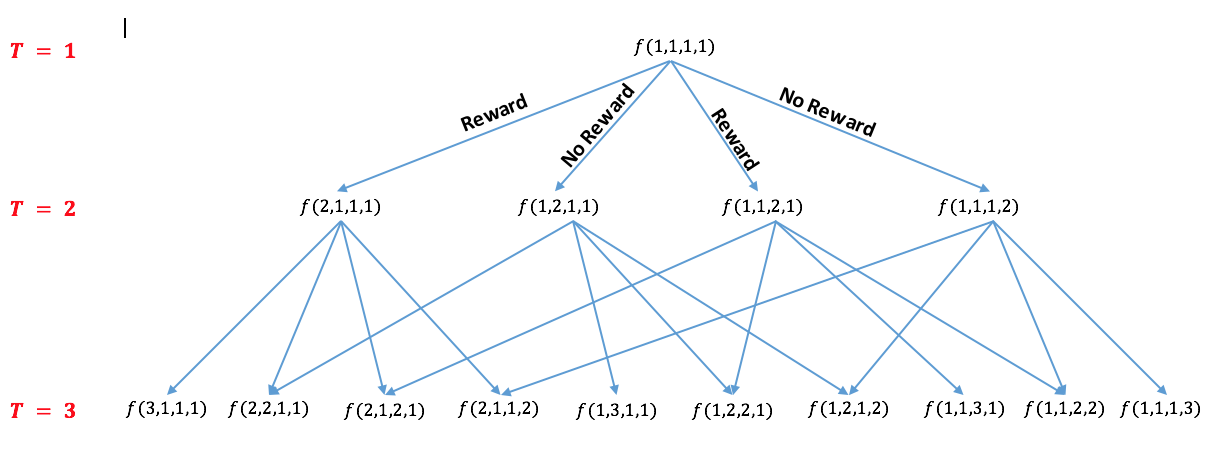
\includegraphics[scale=0.5]{Dynamic_Programming_Tree.png}
\caption{Forest of Possible Outcomes}
\end{figure}

As time increases, the complexity of possible branches increase exponentially, but it is important to note that some branches merge back together. Visually, our algorithm takes in two pieces of information:

1. Current parameters of the Machine based on previous observations
2. Number of Trials we expect to perform

Again, the goal is to maximize the expected future sum of rewards based on the current parameters and the number of future trials. Our algorithm creates a tree of all possible future states, like above, and dynamically works backwards, assuming at the final stage we want to be completely greedy (since it is our last trial). The output is which Machine to play at the current stage, as well as the expected sum of rewards given you follow the algorithm at each trial.

One might assume that we would be greedy at every approach, but our algorithm proves otherwise. It bases its decision on expected future rewards, and it is interesting to see it choose the Machine with the lower expected reward, based on its future possible states.

\subsection{$\epsilon$-greedy}

- Sunith

\subsection{Upper Confidence Bounds}

The other algorithms presented in this paper are similar in that they pay attention only to how much reward they’ve gotten from the machines. This means that they're likely to under-explore options whose initial experiences were not rewarding, even though they may not have enough data to be confident about those arms. One naive approach to solving this problem is to run the algorithm multiple times and take the average of the results. Another could be to run the algorithm for a very long time and hope the probabilistic nature will eventually correct for random variation in the reward distribution. Another approach is to use probability theory to bound our confidence in how good or bad each machine is. This is exactly what Upper Confidence Bounds does.\\

The upper confidence bound (UCB) family of algorithms selects the machine with the largest upper confidence bound at each round. This paper will only focus on UCB1, but note that there are many variants of the UCB family. The more times you play a machine, the tighter the confidence bounds become. So as the number of plays for each machine increases, the uncertainty decreases, and so does the width of the confidence bound.\\

We want to know with high probability that the true expected payoff of a play $\hat{\mu_i}$ is less than our prescribed upper bound:

$$\bar{\mu_{i}} + \sqrt{\frac{2 ln (t)}{n_i}}$$

Where $\bar{\mu_{i}}$ is the average reward obtained from machine $i$ and $n_i$ is the number of times machine $i$ has been played so far.\\

This upper bound is the sum of two terms, where:

\begin{enumerate}
\item the first term is the average reward
\item the second term is related to the one-sided confidence interval for the average reward according to the Chernoff-Hoeffding bounds
\end{enumerate}

Recall that since rewards follow a Bernoulli distribution, we can apply Chernoff-Hoeffding to upper bound the probability that the sum of rewards from each machine deviates from its expected value:

$$\displaystyle \textup{P}(Y + a < \mu) \leq e^{-2na^2}$$

This confidence bound grows with the total number of actions we have taken but shrinks with the number of times we have tried this particular action. This ensures each action is tried infinitely often but still balances exploration and exploitation. It can be shown that the regret for UCB1 grows with \textbf{ln n}, as witnessed below for the optimal machine.\\

Note that in addition to keeping track of our confidence in the estimated values of each machine, the UCB algorithm doesn’t use randomness at all. Unlike the other algorithms in this paper (and in the literature) it’s possible to know exactly how UCB will behave in any given situation. This can make it easier to reason about at times.

\subsubsection{UCB1: Algorithm}

Assuming $K$ machines:

\begin{enumerate}
\item Play each arm once
\item Observe rewards $r_i$, for $i = 1, ..., K$
\item Set $n_i = 1$, for $i = 1, ..., K$
\item set $\bar{\mu_{i}} = \frac{r_i}{n_i}$
\item For time $t = K+1, ..., N$:
	\begin{enumerate}
		\item Play arm $\hat{i} = \underset{i}{\text{argmax}}\text{ }(\hat{\mu_{i}} + \sqrt{\frac{2 ln (t)}{n_i}})$
		\item Observe reward $r$
		\item $r_{\hat{i}} = r_{\hat{i}} + r$
		\item $n_{\hat{i}} = n_{\hat{i}} + 1$
		\item update $\hat{\mu_{i}} = \frac{r_{\hat{i}}}{n_{\hat{i}}}$
	\end{enumerate}
\end{enumerate}

Below we run UCB1 on 5 machines with true reward distribution, $[0.05,0.1,0.3,0.2,0.5]$:

\begin{figure}[H]
\centering
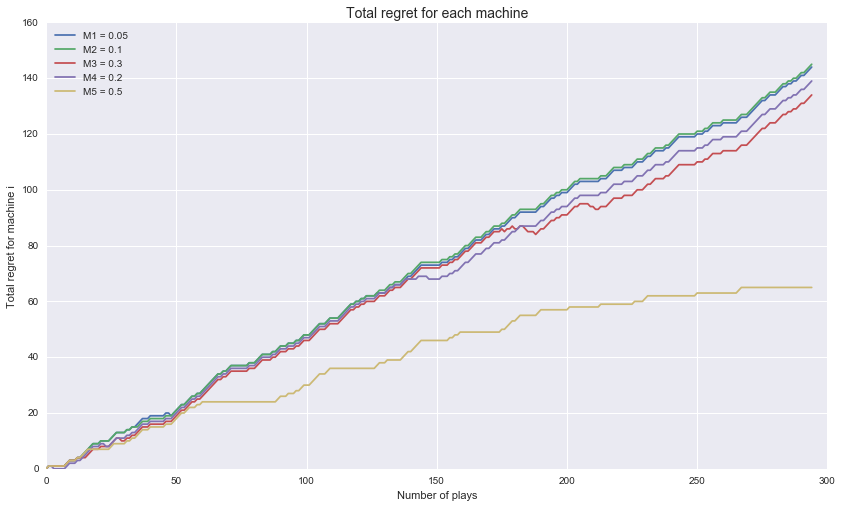
\includegraphics[scale=0.5]{UCB_regret.png}
\caption{Cumulative Regret}
\end{figure}


\begin{figure}[H]
\centering
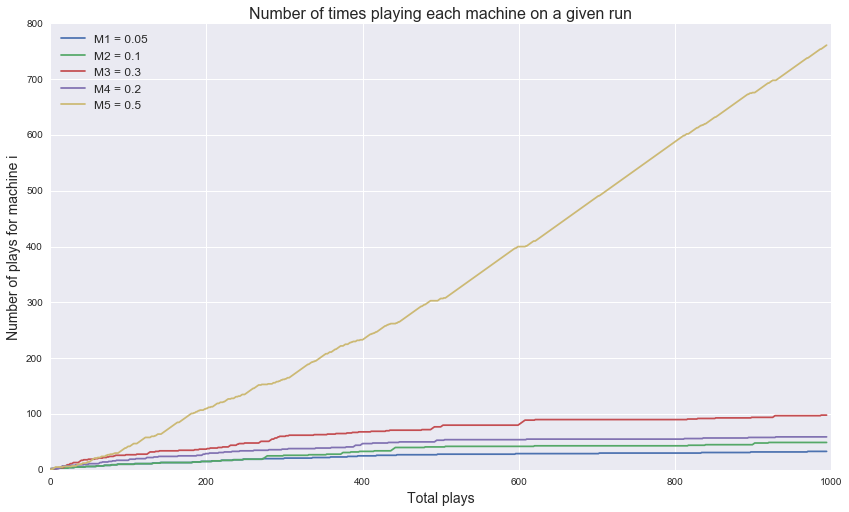
\includegraphics[scale=0.5]{UCB_num_plays.png}
\caption{Switching between machines}
\end{figure}

\textbf{<<<<<<<INSERT COMMENTARY>>>>>>>>>}

\section{Bayesian approaches}

\subsection{Bernoulli Bandit}

Another popular approach to solving the MAB problem is to minimize regret using Bayesian inference. In the above sections, we assumed that rewards were distributed as a Bernoulli with some latent parameter, $\theta_i$, specific to each machine. However we didn't make this explicit. The Bayesian approach is to put a prior distribution on $\theta_i$ and update that belief as we run the algorithm and learn which machines are better than others. Since rewards are generated from a Bernoulli distribution, a natural choice for the distribution on $\theta_i$ is a Beta. Formally:

$$\theta_i \sim \text{Beta}(\alpha_i, \beta_i)$$
$$r_i = \text{Reward from Machine i} \sim \text{Bernoulli}(\theta_i)$$

Exploiting the conjugacy of the Beta-Bernoulli model, the posterior distribution of getting a reward from $\text{machine}_i$, after playing for $N$ iterations is:
$$\text{Beta}(\alpha_i + R_{N}, \beta_i + T - R_{N})$$

where $R_{N} = \sum_{t=1}^{N}r_{t}$.\\

Before beginning to play, we assume no prior knowledge about any machine's propensity to yield a positive reward. Therefore, we initially set $\alpha_i, \beta_i = 1$, which is a common objective prior for the Beta distribution.\\

\subsection{Thompson Sampling}

The generic algorithm used for Bayesian inference is as follows:

\begin{enumerate}
\item For $t = 1, ..., N$
\item U($\alpha_i$, $\beta_i$) = $i_t$  // select machine $i$ at time $t$ using the policy/acquisition function
\item $r_t \sim \text{Bernoulli}(\theta_{i})$  i  // We play Machine $i$, and get Reward $r_t$
\item If $r_t = 1: \alpha_i = \alpha_i + 1$   // if the reward was successful, increase our positive belief in machine $i$
\item else if $r_t = 0: \beta_i = \beta_i + 1$  // if we didn't get a reward, increase our negative belief (i.e. failure) in machine $i$
\item $R_t = R_t + r_t$		// add reward at time $t$ to running total
\end{enumerate}

This algorithm provides a framework for how to think about this problem in a Bayesian way. To maximize expected rewards, we must optimally choose the policy function U.\\

Note that we don't really care about how accurate we become about inferences of the hidden probabilities, $\theta_i$ - for this problem we are more interested in choosing the best bandit that maximizes rewards.

Below we explore 3 ways to select the policy:

\begin{enumerate}
\item \textbf{Explore}: Randomly select one of the $K$ machines, without considering how many win/losses you've seen. This is a pure eploratory strategy and is used for comparison purposes only.
\item \textbf{Exploit}: Sample each $\theta_i \sim Beta(\alpha_i, \beta_i)$. Select $\underset{i}{\text{argmax}}\text{ }\mathbf{E}[\theta_i]$. This is called {"Exploit"} because we are greedily choosing the best machine at each step based on expected rewards. Note however that even if we select the best expected machine, there is a non-zero probability ($\frac{\beta_i}{\alpha_i + \beta_i}$) that it fails to generate a reward. So the amount of exploration is small but non-zero. Also note that this approach is sometimes called \text{"Adbandit"}.
\item \textbf{Thompson-Sampling}: Sample each $\theta_i \sim Beta(\alpha_i, \beta_i)$. Select $\underset{i}{\text{argmax}}\text{ }\theta_i$. This approach falls somewhere between Exploit and Explore, but is much closer to Exploit. In expectation we expect Thompson-Sampling to be very close to Exploit.
\end{enumerate}

Below we present comparisons of the three approaches using the same dataset as above for UCB:

\begin{figure}[H]
\centering
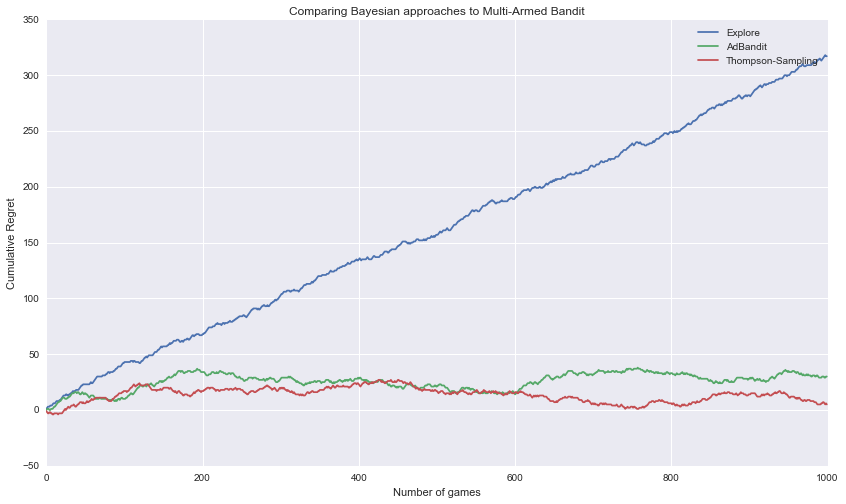
\includegraphics[scale=0.5]{Bayesian_regret.png}
\caption{Cumulative Regret}
\end{figure}

\subsection{Gaussian Process and Reinforcement Learning}

- Lin
\begin{itemize}
\item assume knowledge of GPs, so no need to explain what a GP is
\item quick overview of how MAB relates to reinforcement learning
\item quick overview of how GPs relate to reinforcement learning
\item using the mechanics of GP, what the connection between GP and MAB is
\item show a chart or two like in the presentation
\item this will be multiple sections
\end{itemize}

\section{Empirical Comparisons}

\subsection{Data set}

\subsection{Charts}

- using the same data set, compare UCB vs. epsilon vs. Thompson vs. gittins vs. GP

\section{Conclusion}

\section{References}


\end{document}
